%&pdflatex
\documentclass[11pt, a4paper]{article}
\usepackage{graphicx}
\usepackage{amsmath}
\usepackage{listings}
\usepackage{minted}
\usepackage{float}

\title{EE2703 Applied Programming Lab - \\Assignment No 4}
\author{
  \textbf{Name}: Abishek S\\
  \textbf{Roll Number}: EE18B001
}\date{\today}
\begin{document}
		
\maketitle 
\section{Abstract}
The goal of this assignment are the following :
\begin{itemize}
\item To find Fourier series coefficients of two functions - $e^{x}$ and $cos(cos(x))$.
\item To estimate Fourier series coefficients using Least square fitting.
\item Studying the effect of discontinuities on the Fourier Series, and the Gibbs Phenomenon.
\item To plot graphs and analyse the above.
\end{itemize}
\usemintedstyle{manni}

\section{Assignment}
The Fourier series is given by :
\begin{equation}\label{eq:fs1}
a_0 + \sum_{n=1}^{\infty} \{a_n cos(nx) + b_n sin(nx)\}
\end{equation}
\subsection{Part 1}
Importing the standard libraries
\begin{minted}[mathescape,escapeinside = ||,tabsize = 4]{python3}
from scipy.integrate import quad
from scipy.linalg import lstsq
import pylab as pl
import numpy as np
import sys
import math
\end{minted}
Defining the original functions $e^{x}$ and $cos(cos(x))$
\begin{minted}[tabsize = 4]{python3}
def exp(x):
	return np.exp(x) if np.isscalar(x) else np.exp(np.array(x))

def coscos(x):
	return np.cos(np.cos(x)) if np.isscalar(x) else np.cos(np.cos(np.array(x)))
\end{minted}
Defining the periodic extension of functions $e^{x}$ and $cos(cos(x))$
\begin{minted}[tabsize = 4]{python3}
def f1(x):
	X = np.asarray([x]) if np.isscalar(x) else np.asarray(x)
	X = list(map(lambda y: y - math.floor(y/(2*np.pi))*(2*np.pi),X))
	return np.exp(X[0]) if np.isscalar(x) else np.exp(np.array(X))

def f2(x):
	X = np.asarray([x]) if np.isscalar(x) else np.asarray(x)
	X = list(map(lambda y: y - math.floor(y/2*np.pi)*(2*np.pi),X))
	return np.cos(np.cos(X[0])) if np.isscalar(x) else np.cos(np.cos(np.array(X)))
\end{minted}

We plot the two functions from $-2\pi$ to $4\pi$ , both the original and periodic extension.
\begin{minted}[tabsize = 4]{python3}
#Plotting exp(x) original and periodic extensions in same graph
pl.figure(1)
pl.title('Original and periodic extension of exp(x)')
pl.semilogy(X_list,exp(X_list),label = 'exp(x) - Original')
pl.semilogy(X_list,f1(X_list),label = 'exp(x) - Periodic Extension')
pl.xlabel(r'X $\rightarrow$')
pl.ylabel(r'Y $\rightarrow$')
pl.legend()
pl.grid(True)
pl.show()

#Plotting exp(x) original and periodic extensions in same graph
pl.figure(2)
pl.title('Original and periodic extension of cos(cos(x))')
pl.plot(X_list,coscos(X_list),label = 'cos(cos(x)) - Original')
pl.plot(X_list,f2(X_list),label = 'cos(cos(x)) - Periodic Extension')
pl.xlabel(r'X $\rightarrow$')
pl.ylabel(r'Y $\rightarrow$')
pl.legend()
pl.grid(True)
pl.show()
\end{minted}

\begin{figure}[H]
   	\centering
   	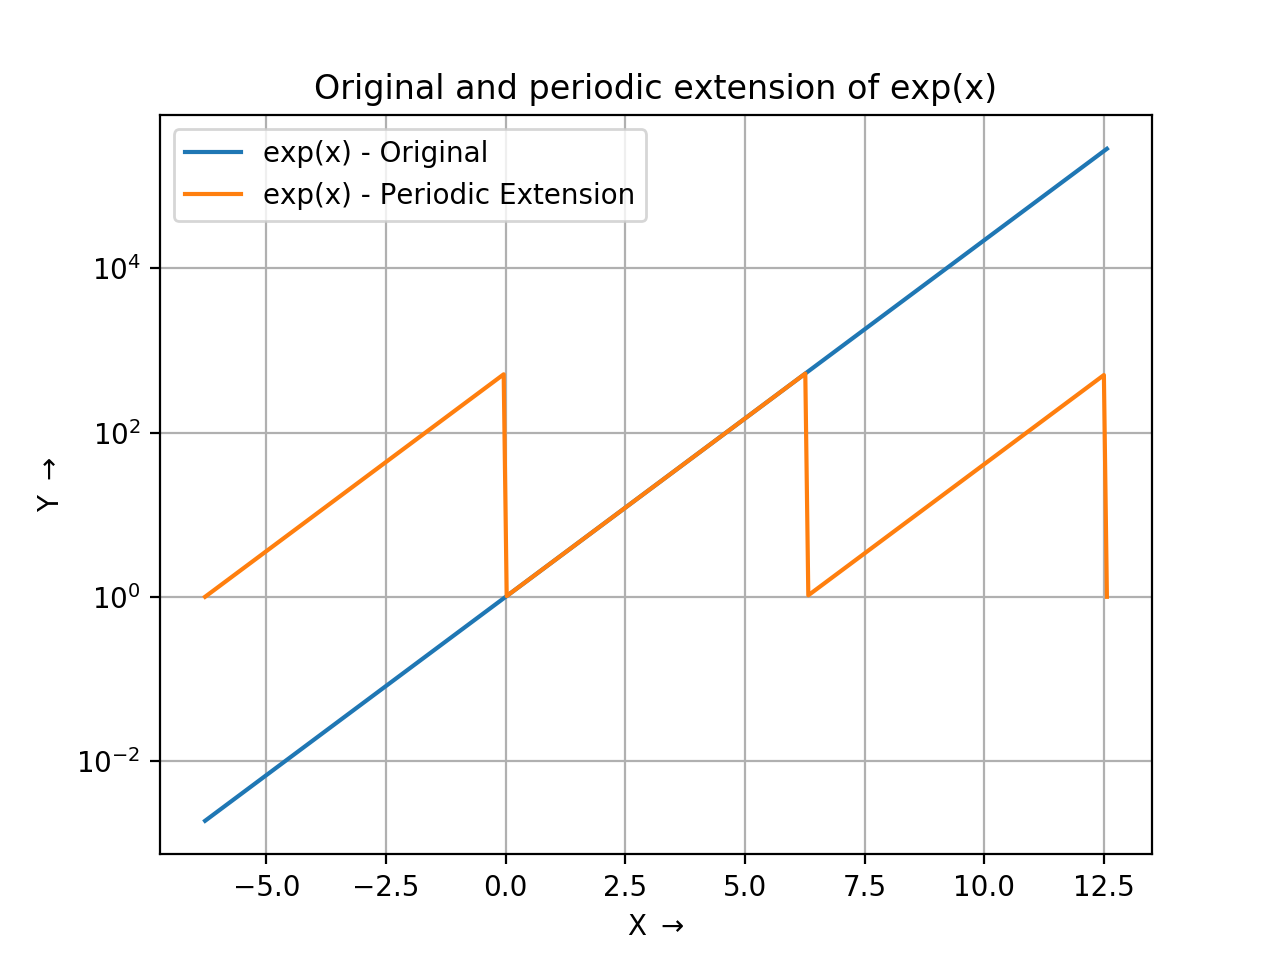
\includegraphics[scale=0.5]{exp.png}
   	\label{fig:exp}
   	\caption{$e^{x}$ vs t on a linear plot}
\end{figure}

\begin{figure}[H]
   	\centering
   	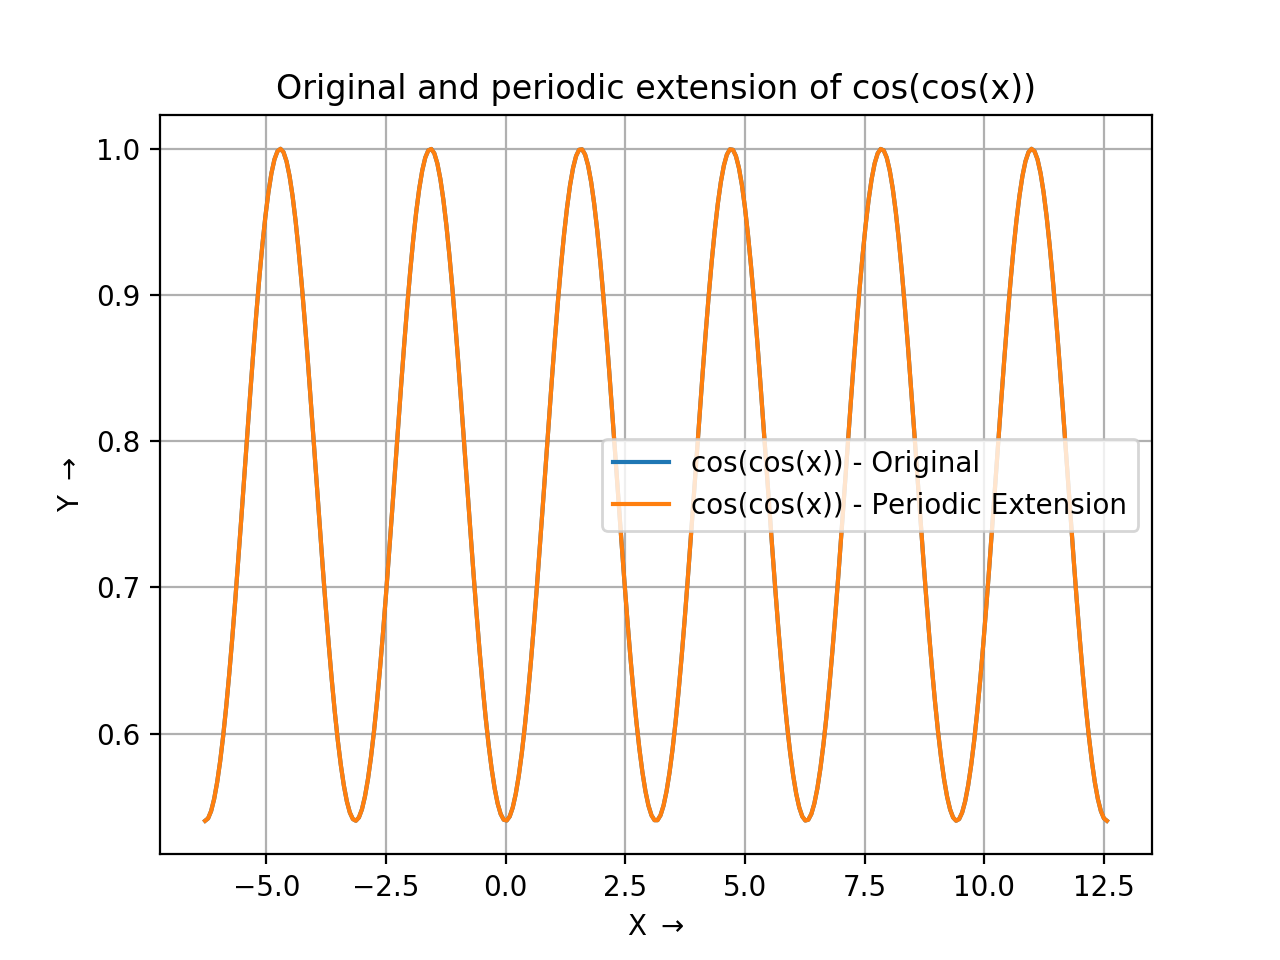
\includegraphics[scale=0.5]{coscos.png}
   	\label{fig:coscos}
   	\caption{$cos(cos(x))$ vs t on a linear plot}
\end{figure}

\subsection{Part 2}
We use the integrator in scipy to calculate the fourier series coefficients through the following formulae :
\begin{equation} \label{eq:1}
\begin{aligned}
&a_0 = \frac{1}{2\pi}\int_{0}^{2\pi} f(x) dx \\ \\
&a_n = \frac{1}{\pi}\int_{0}^{2\pi} f(x)cos(nx) dx \\ \\
&b_n = \frac{1}{\pi}\int_{0}^{2\pi} f(x)sin(nx) dx
\end{aligned}
\end{equation}
\begin{minted}[tabsize = 4]{python3}
def u(x,k,f):
	return f(x)*np.cos(k*x)

def v(x,k,f):
	return f(x)*np.sin(k*x)

a = np.zeros((2,26))
b = np.zeros((2,26))

for i in range(26):
	a[0][i] = quad(u,0,2*np.pi,args=(i,f1))[0]/np.pi
	if(i == 0):
		a[0][i] /= 2

for i in range(26):
	b[0][i] = quad(v,0,2*np.pi,args=(i,f1))[0]/np.pi
	if(i == 0):
		b[0][i] /= 2

for i in range(26):
	a[1][i] = quad(u,0,2*np.pi,args=(i,f2))[0]/np.pi
	if(i == 0):
		a[1][i] /= 2

for i in range(26):
	b[1][i] = quad(v,0,2*np.pi,args=(i,f2))[0]/np.pi
	if(i == 0):
		b[1][i] /= 2
\end{minted}

\subsection{Part 3}
We plot the Fourier series coefficients - in loglog anf semilog plots.
The numbering of coefficients is given by 1-indexing the vector :
$$
\begin{pmatrix}
a_0 \\
a_1 \\
b_1 \\
... \\
a_{25} \\
b_{25} \\
\end{pmatrix}
$$
\begin{minted}[tabsize = 4]{python3}
pl.figure(3)
pl.title('Loglog Fourier coefficients of exp(x)')
pl.loglog(np.arange(0,51,1),np.absolute(C[0]),'ro',label = 'exp(x)')
pl.xlabel(r'log n $\rightarrow$')
pl.ylabel(r'log of Magnitude of coefficient $\rightarrow$')
pl.legend()
pl.grid(True)
pl.show()

pl.figure(4)
pl.title('Semilogy Fourier coefficients of exp(x)')
pl.semilogy(np.arange(0,51,1),np.absolute(C[0]),'ro',label = 'exp(x)')
pl.xlabel(r'n $\rightarrow$')
pl.ylabel(r'log of Magnitude of coefficient $\rightarrow$')
pl.legend()
pl.grid(True)
pl.show()

pl.figure(5)
pl.title('Loglog Fourier coefficients of cos(cos(x))')
pl.loglog(np.arange(0,51,1),np.absolute(C[1]),'ro',label = 'cos(cos(x))')
pl.xlabel(r'log n $\rightarrow$')
pl.ylabel(r'log of Magnitude of coefficient $\rightarrow$')
pl.legend()
pl.grid(True)
pl.show()

pl.figure(6)
pl.title('Semilogy Fourier coefficients of cos(cos(x))')
pl.semilogy(np.arange(0,51,1),np.absolute(C[1]),'ro',label = 'cos(cos(x))')
pl.xlabel(r'n $\rightarrow$')
pl.ylabel(r'log of Magnitude of coefficient $\rightarrow$')
pl.legend()
pl.grid(True)
pl.show()
\end{minted}

\begin{figure}[H]
   	\centering
   	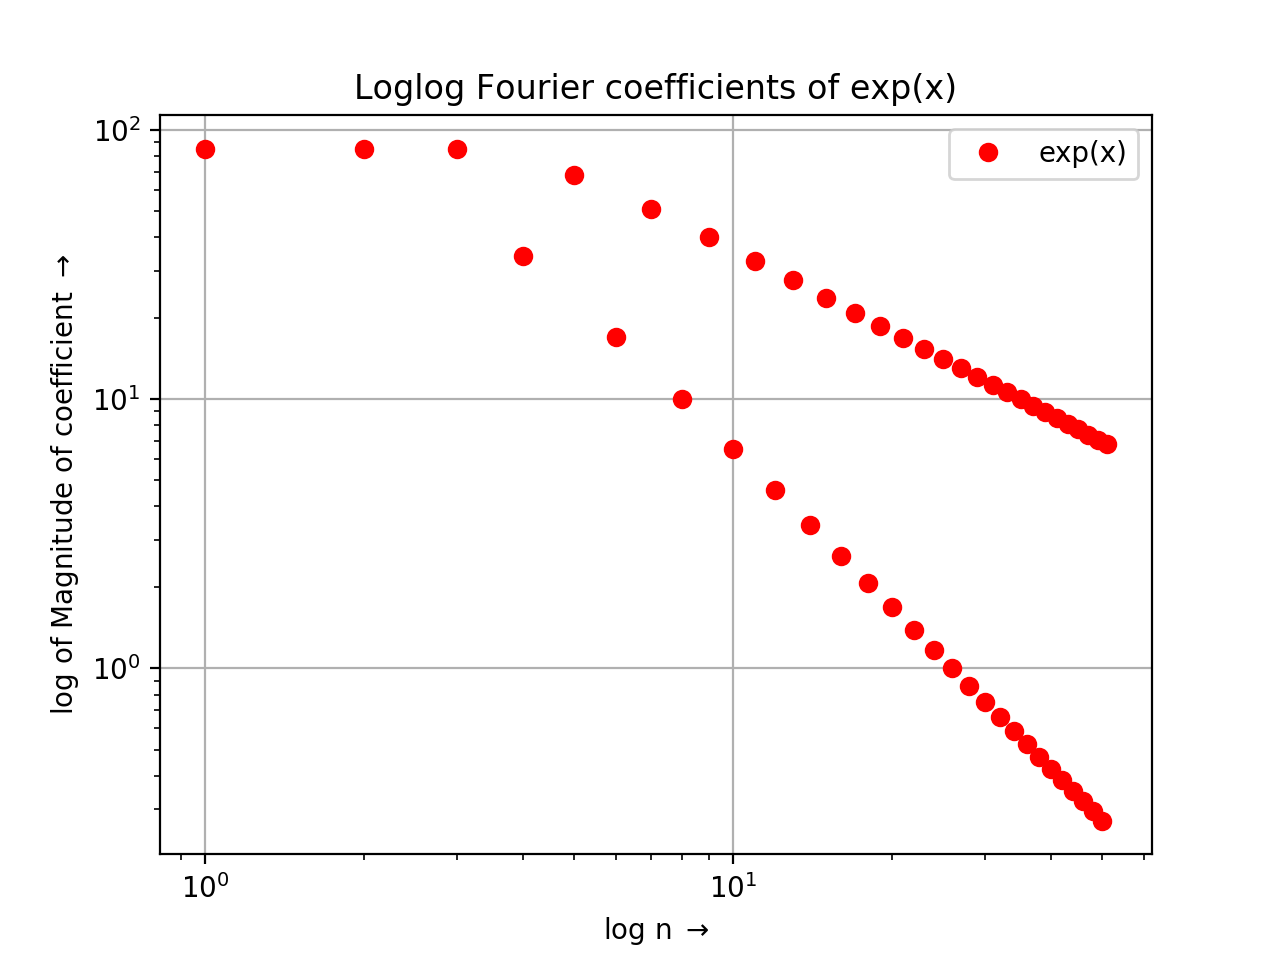
\includegraphics[scale=0.5]{loglog1t.png}
   	\label{fig:loglog1t}
   	\caption{Coefficients of $e^{x}$ by Integration- Loglog Plot}
\end{figure}
\begin{figure}[H]
   	\centering
   	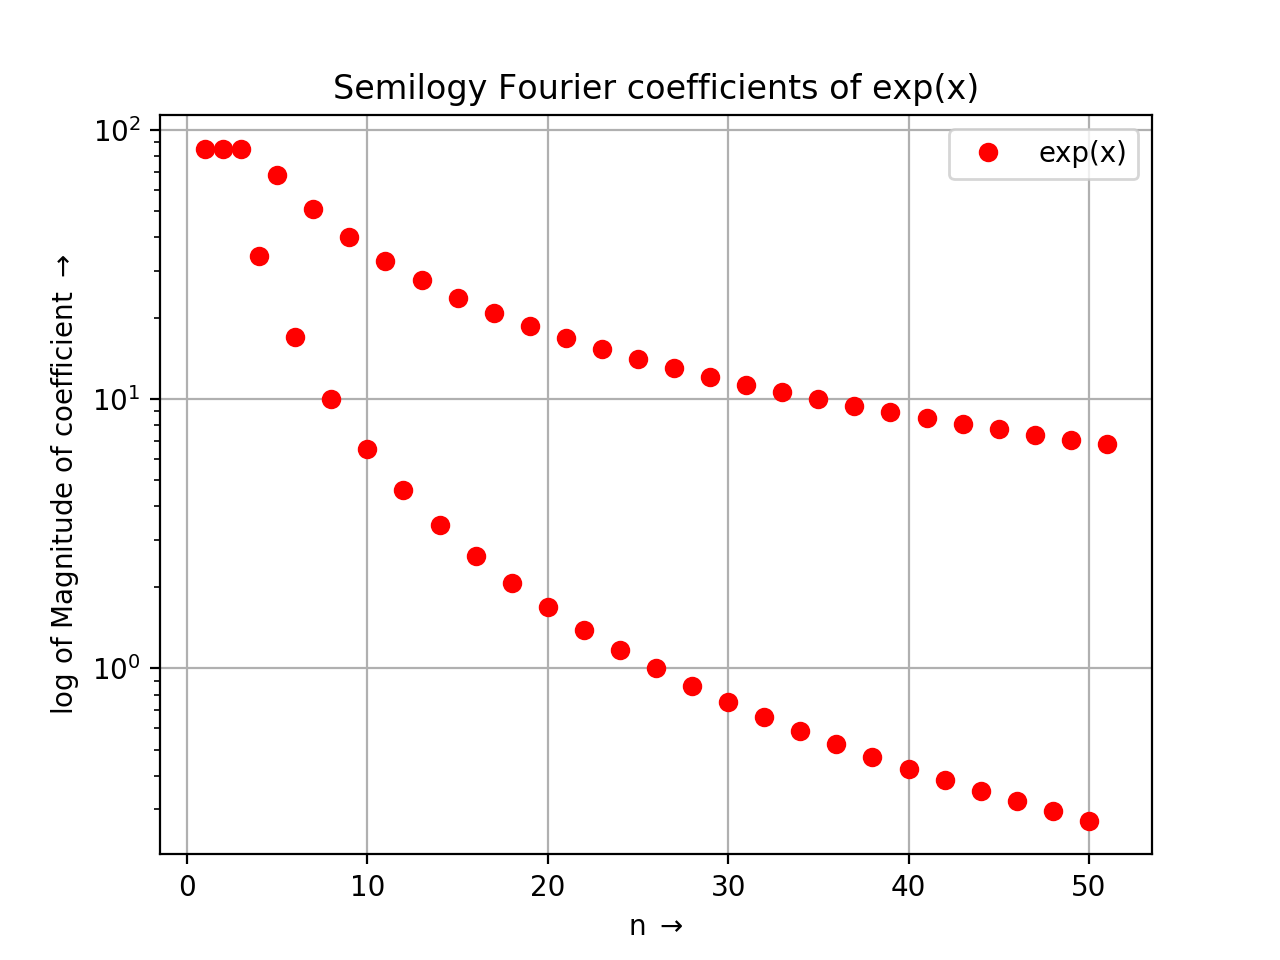
\includegraphics[scale=0.5]{semilog1t.png}
   	\label{figsemilog1t}
   	\caption{Coefficients of $e^{x}$ by Integration- Semilog Plot}
\end{figure}
   
\begin{figure}[H]
   	\centering
   	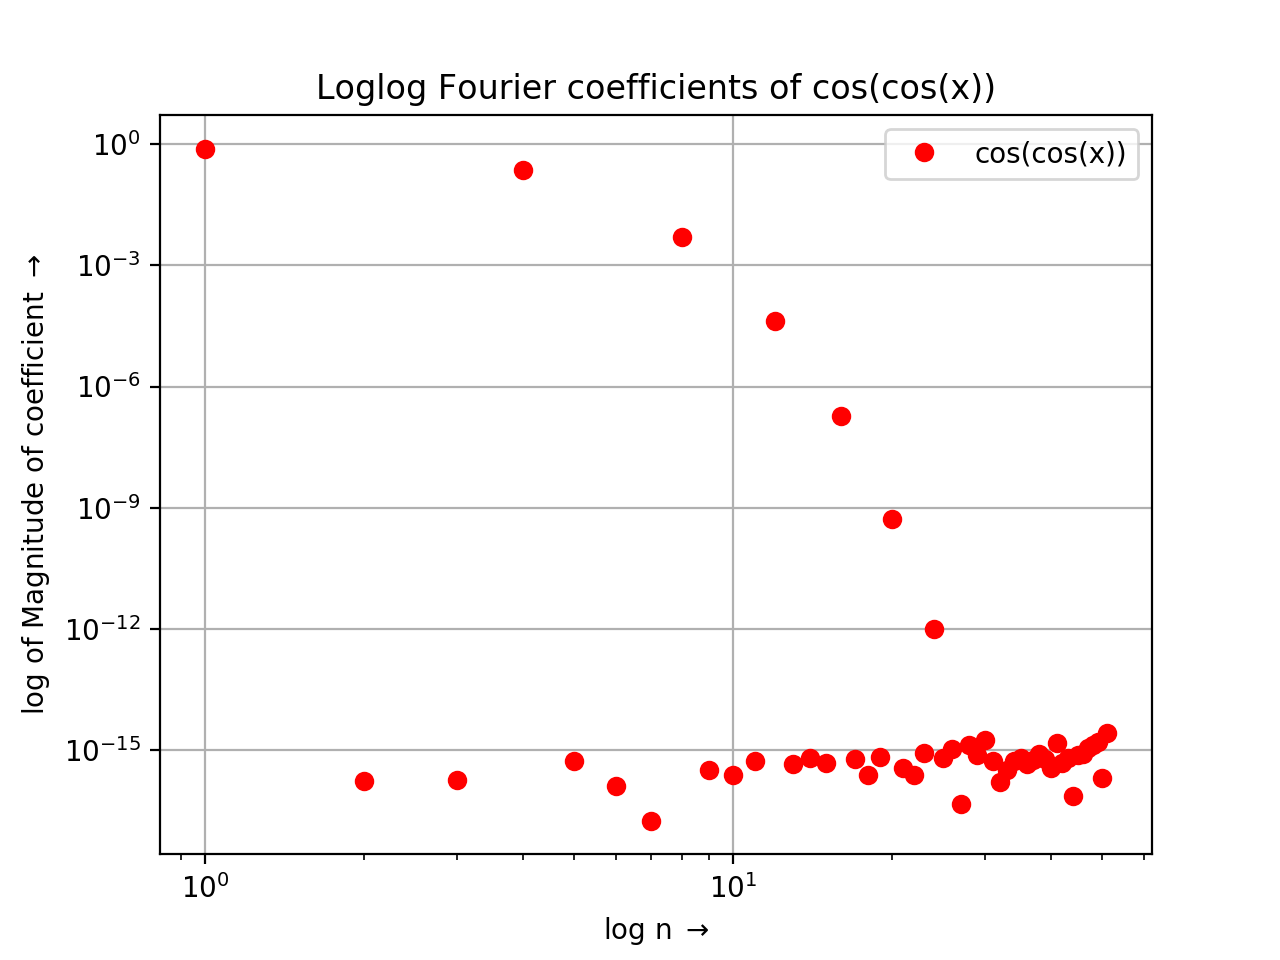
\includegraphics[scale=0.5]{loglog2t.png}
   	\label{fig:loglog2t}
   	\caption{Coefficients of $cos(cos(x))$ by Integration- Loglog Plot}
\end{figure}

\begin{figure}[H]
   	\centering
   	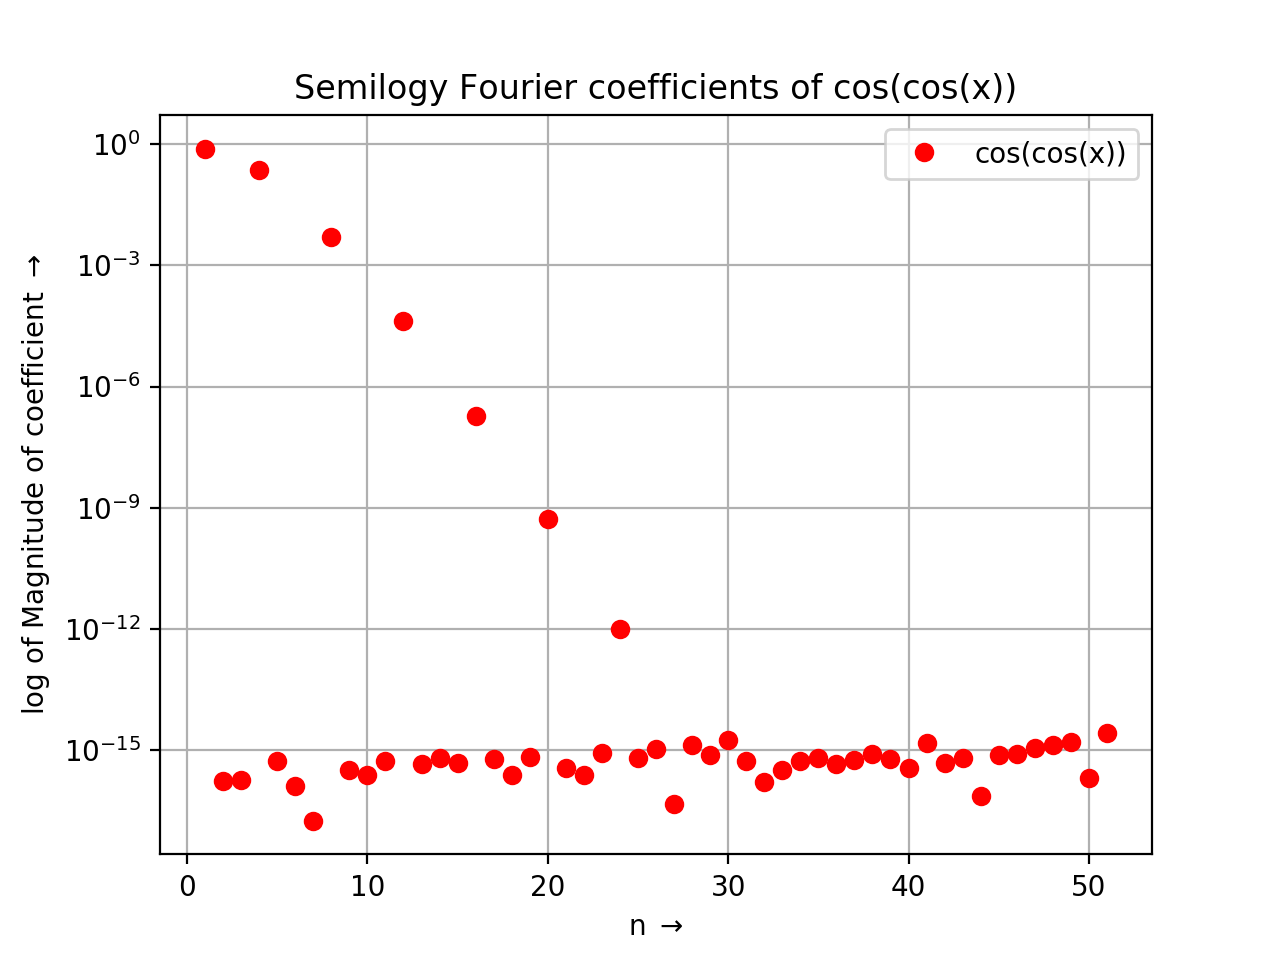
\includegraphics[scale=0.5]{semilog2t.png}
   	\label{fig:semilog2t}
   	\caption{Coefficients of $cos(cos(x))$ by Integration- Semilog Plot}
\end{figure}

{$a.$ The $b_{n}$ coefficients are nearly zero since $cos(cos(x))$ is an even function, and hence has zero coefficients for the sin (odd function) components.}
\\
{$b.$ The magnitude of the coefficients represents how much of certain frequencies are present in the output. $cos(cos(x))$ does not have many frequencies of harmonics, so it dies out quickly. However, since the periodic extension of $e^{x}$ is discontinuous, to represent this discontinuity as a sum of continuous sinusoids, we would need high frequency components, hence coefficients do not decay as quickly.}
\\
{$c.$ The loglog plot is linear for $e^{x}$ since Fourier coefficients of $e^{x}$ decay with $1/n$ or $1/n^{2}$. The semilog plot seems linear for $cos(cos(x))$ case as its fourier coefficients decay exponentially with n.
}

\subsection{Parts 4 and 5}
We now use least squares method to calculate the Fourier series coefficients and plot them along with the true ones predicted by the integral.
\\
We need :
\begin{equation}\label{eq:fs2}
a_0 + \sum_{n=1}^{25} \{a_n cos(nx_i) + b_n sin(nx_i)\} = f(x_i)
\end{equation}
\begin{equation}\label{eq:2}
\begin{pmatrix}
1 & cosx_1 & sinx_1 & ... & cos25x_1 & sin25x_1 \\
1 & cosx_2 & sinx_2 & ... & cos25x_2 & sin25x_2 \\
... & ... & ... & ... & ... & ... \\
1 & cosx_{400} & sinx_{400 }& ... & cos25x_{400} & sin25x_{400} \\
\end{pmatrix}
\begin{pmatrix}
a_0 \\ a_1 \\ b_1 \\ ... \\ a_{25} \\ b_{25}
\end{pmatrix}
=
\begin{pmatrix}
f(x_1) \\ f(x_2) \\ ... \\ f(x_{400})
\end{pmatrix}
\end{equation}
Notice that here I have specified the endpoint ($2\pi$) of periodic extension of exp(x) as the left limit value. This is done since the fourier series converges to the midpoint of left hand and right hand limits at points of discontinuities. According to the function we defined, the value at $2\pi$ would be that at $0$ (periodic extension), but if we use the same, the Least square approach would estimate the function would reach zero from point before the $2\pi$ point in the sample, and since the sampling rate is low, the prediction would be quite bad. Only if we give value at endpoint like we defined, the function would be nearly discontinuous, and it would converge to the midpoint like what Fourier Series does.
\\
In short, to make sure coefficients predicted by least square approach match with that by integration, I have done the same.
\begin{minted}[tabsize = 4]{python3}
x=pl.linspace(0,2*np.pi,400,endpoint = True)
b1=f1(x) 
b2=f2(x)
#Providing the endpoint for f1(x) alone
b1[-1] = exp(2*np.pi)
A=np.zeros((400,51))
A[:,0]=1
for k in range(1,26):
	A[:,2*k-1]=np.cos(k*x) 
	A[:,2*k]=np.sin(k*x) 
	
c1=lstsq(A,b1)[0]
c2=lstsq(A,b2)[0]

pl.figure(3)
pl.title('Loglog Fourier coefficients of exp(x)')
pl.loglog(np.arange(1,52,1),np.absolute(C[0]),'ro',label = 'True')
pl.loglog(np.arange(1,52,1),np.absolute(c1),'go',label = 'Predicted')
pl.xlabel(r'log n $\rightarrow$')
pl.ylabel(r'log of Magnitude of coefficient $\rightarrow$')
pl.legend()
pl.grid(True)
pl.show()

pl.figure(4)
pl.title('Semilogy Fourier coefficients of exp(x)')
pl.semilogy(np.arange(1,52,1),np.absolute(C[0]),'ro',label = 'True')
pl.semilogy(np.arange(1,52,1),np.absolute(c1),'go',label = 'Predicted')
pl.xlabel(r'n $\rightarrow$')
pl.ylabel(r'log of Magnitude of coefficient $\rightarrow$')
pl.legend()
pl.grid(True)
pl.show()

pl.figure(5)
pl.title('Loglog Fourier coefficients of cos(cos(x))')
pl.loglog(np.arange(1,52,1),np.absolute(C[1]),'ro',label = 'True')
pl.loglog(np.arange(1,52,1),np.absolute(c2),'go',label = 'Predicted')
pl.xlabel(r'log n $\rightarrow$')
pl.ylabel(r'log of Magnitude of coefficient $\rightarrow$')
pl.legend()
pl.grid(True)
pl.show()

pl.figure(6)
pl.title('Semilogy Fourier coefficients of cos(cos(x))')
pl.semilogy(np.arange(1,52,1),np.absolute(C[1]),'ro',label = 'True')
pl.semilogy(np.arange(1,52,1),np.absolute(c2),'go',label = 'Predicted')
pl.xlabel(r'n $\rightarrow$')
pl.ylabel(r'log of Magnitude of coefficient $\rightarrow$')
pl.legend()
pl.grid(True)
pl.show()
\end{minted}

\begin{figure}[H]
   	\centering
   	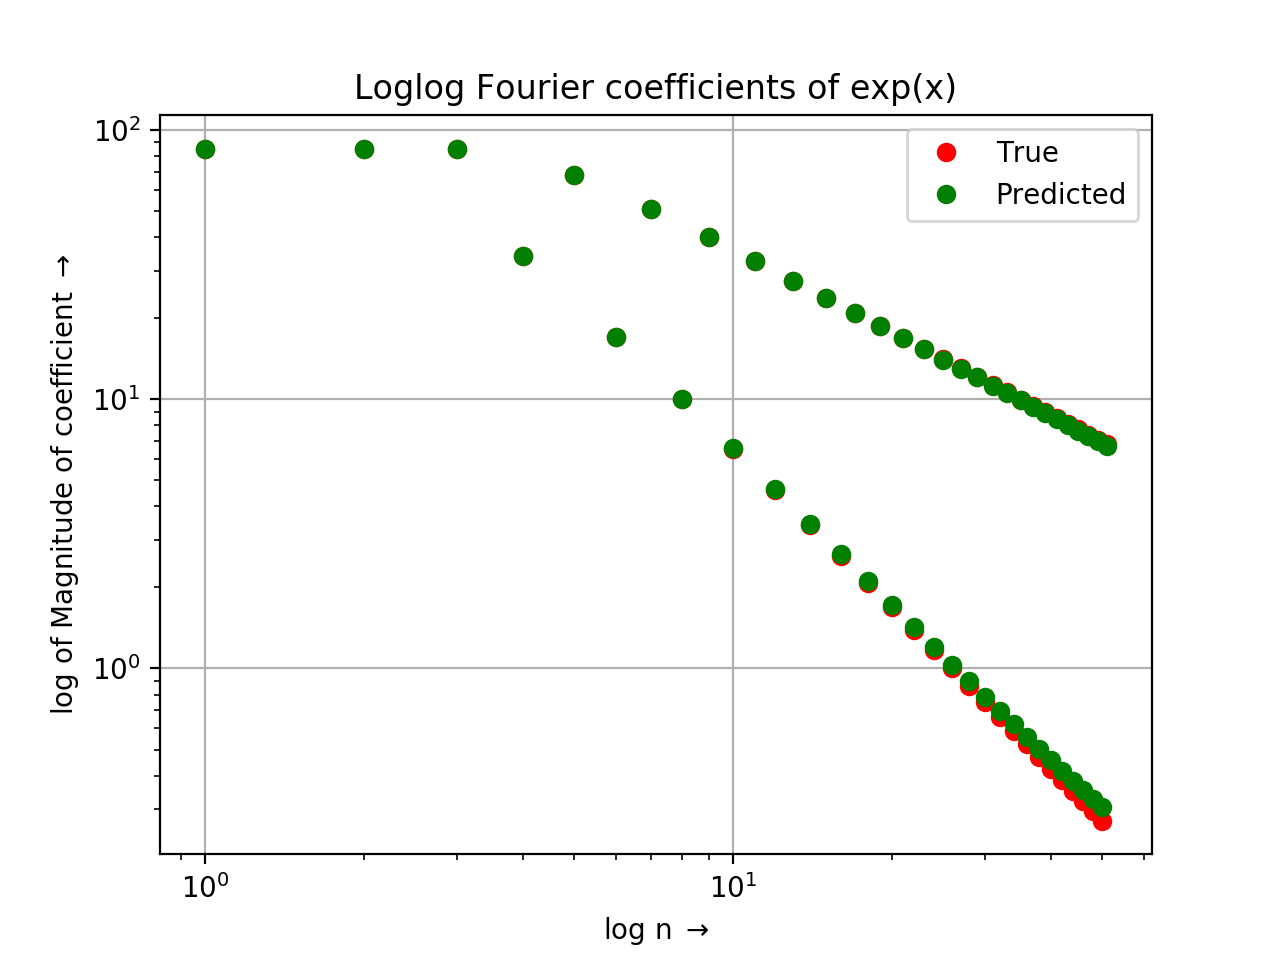
\includegraphics[scale=0.5]{loglog1p.png}
   	\label{fig:loglog1p}
   	\caption{Coefficients of $e^{x}$ with discontinuity correction - Loglog Plot}
\end{figure}
\begin{figure}[H]
   	\centering
   	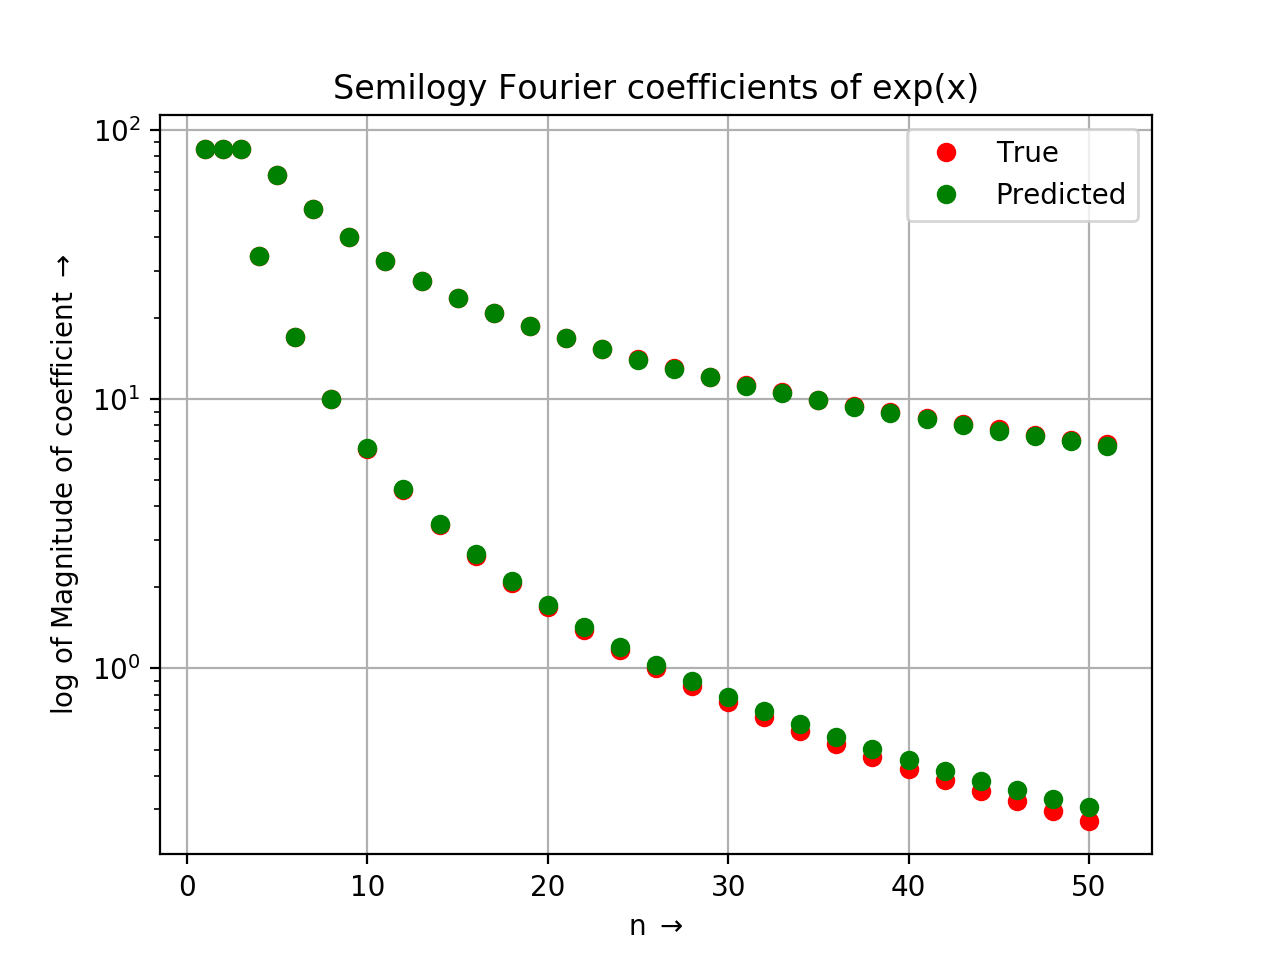
\includegraphics[scale=0.5]{semilog1p.png}
   	\label{fig:semilog1p}
   	\caption{Coefficients of $e^{x}$ with discontinuity correction - Semilog Plot}
\end{figure}
\begin{figure}[H]
   	\centering
   	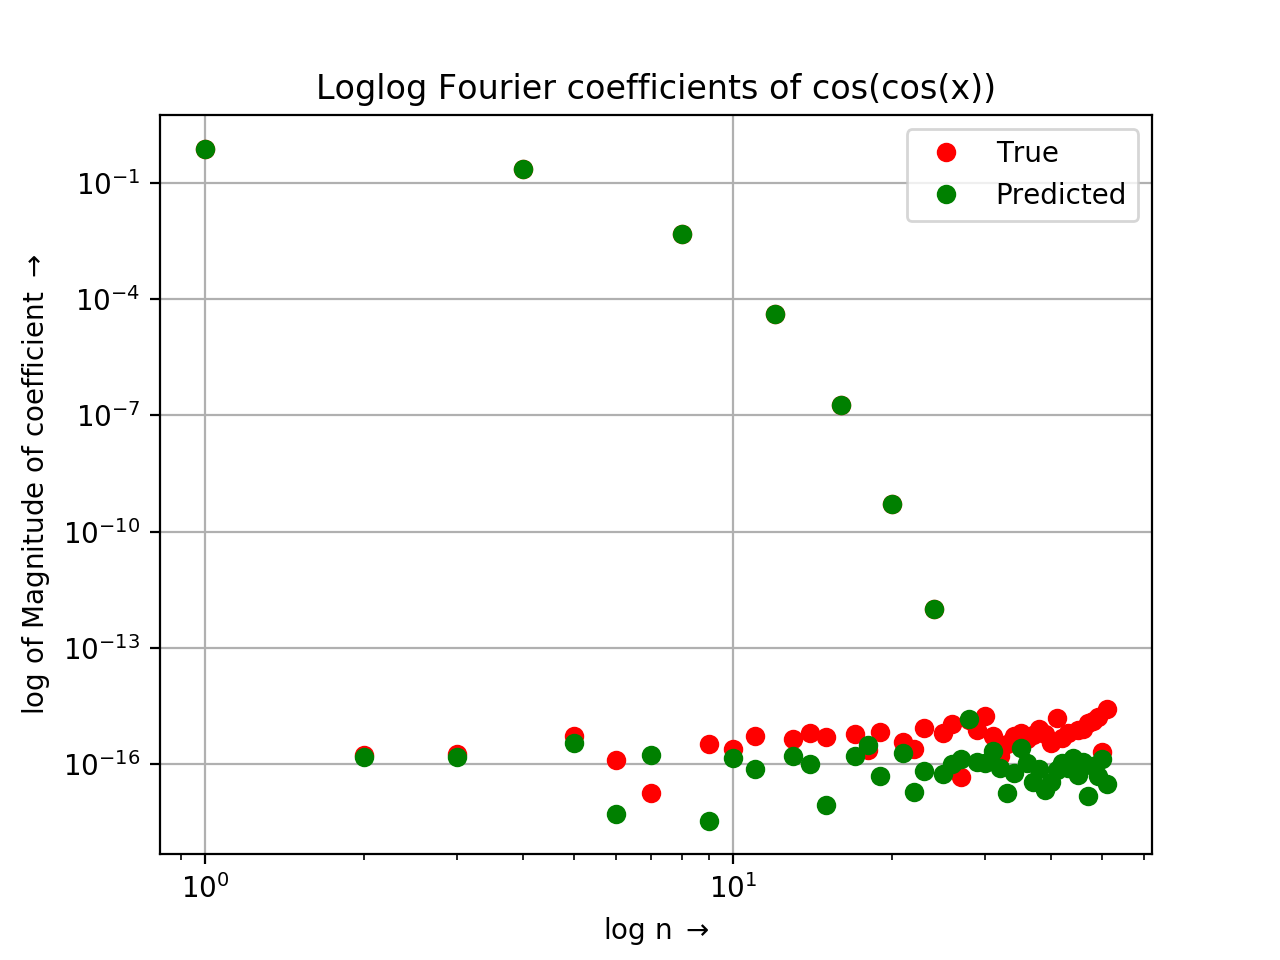
\includegraphics[scale=0.5]{loglog2p.png}
   	\label{fig:loglog2p}
   	\caption{Coefficients of $cos(cos(x))$ - Loglog Plot}
\end{figure}
\begin{figure}[H]
   	\centering
   	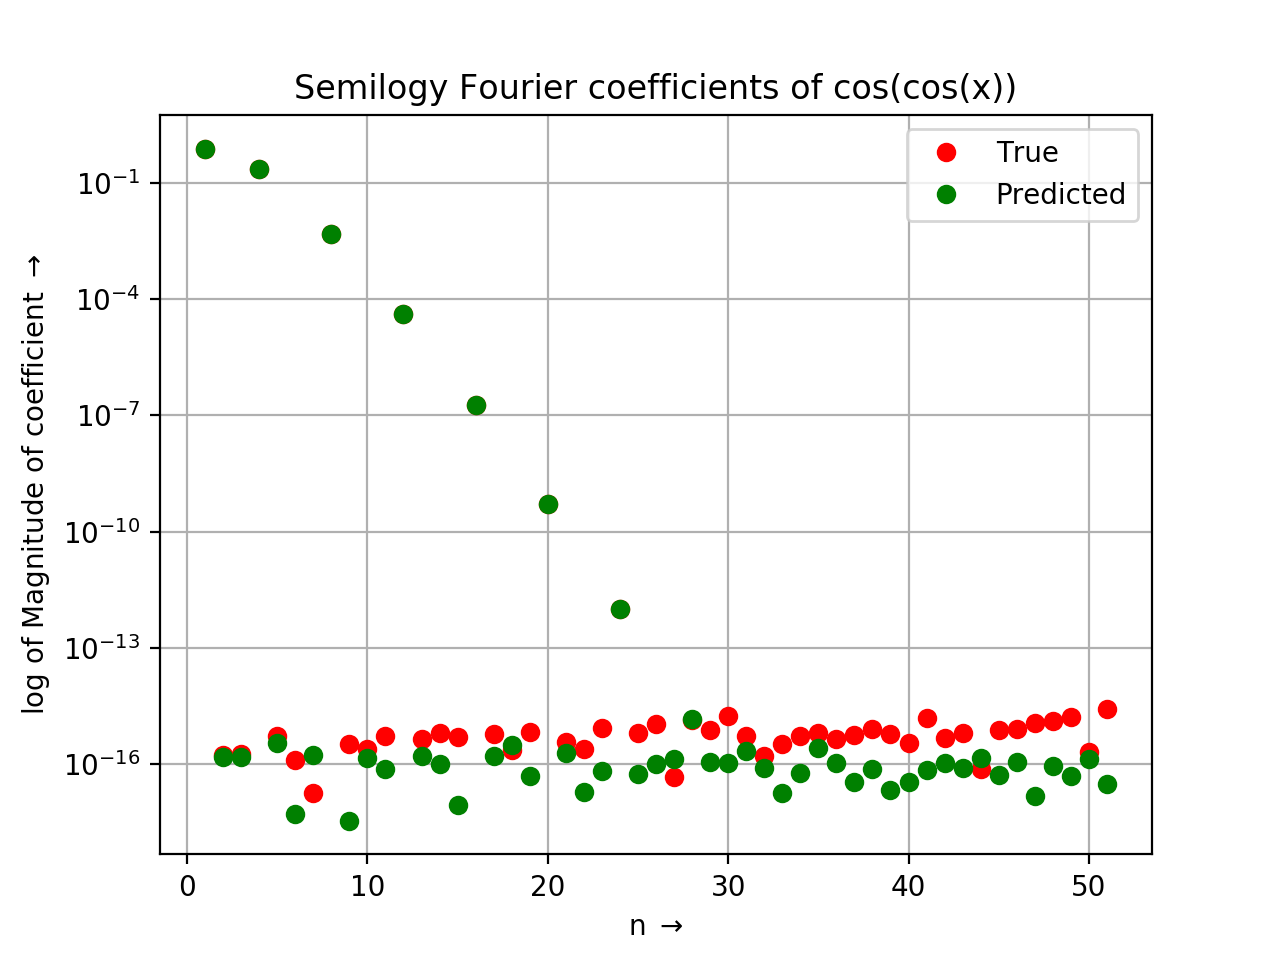
\includegraphics[scale=0.5]{semilog2p.png}
   	\label{fig:semilog2p}
   	\caption{Coefficients of $cos(cos(x))$ - Semilog Plot}
\end{figure}
Incase I did not specify the endpoint of the periodic extension of function exp(x), the plots would become the following, because of the difference in the values predicted at the discontinuity by the least square method and the integration method.

\begin{figure}[H]
   	\centering
   	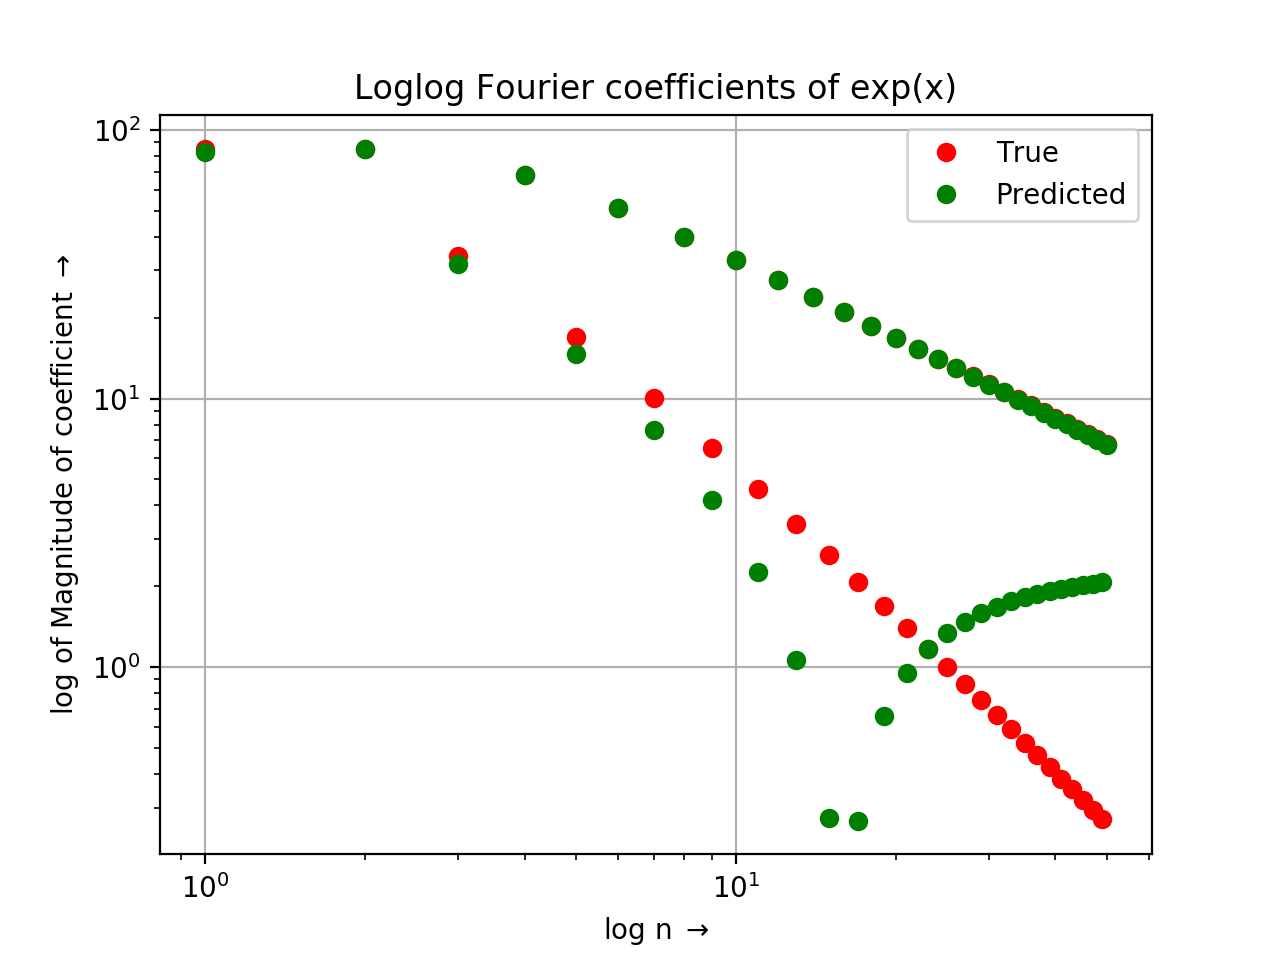
\includegraphics[scale=0.5]{loglog1e.png}
   	\label{fig:loglog1e}
   	\caption{Coefficients of $e^{x}$ without discontinuity correction - Loglog Plot}
\end{figure}
\begin{figure}[H]
   	\centering
   	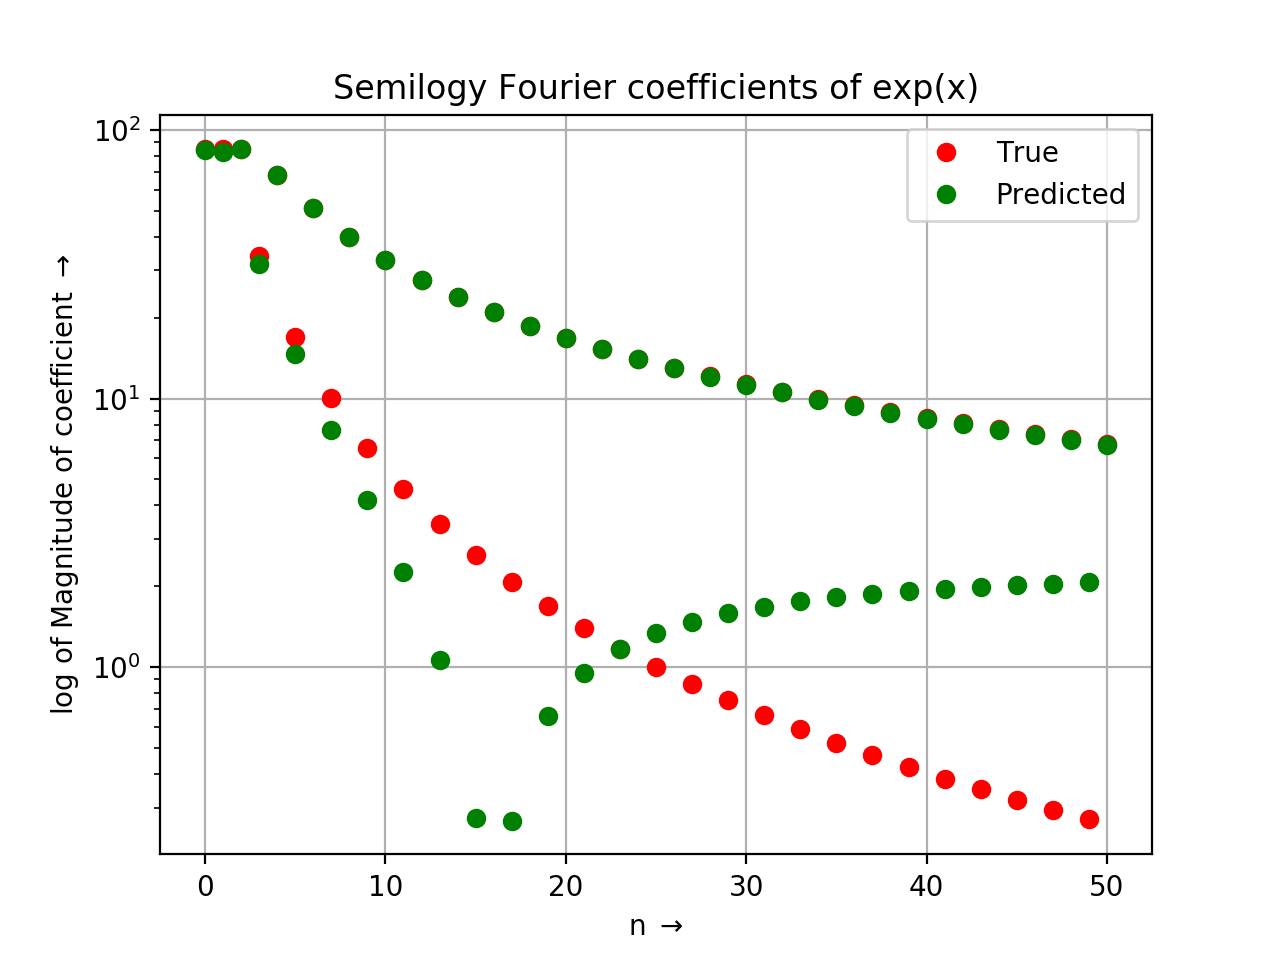
\includegraphics[scale=0.5]{semilog1e.png}
   	\label{fig:semilog1e}
   	\caption{Coefficients of $e^{x}$ without discontinuity correction - Semilog Plot}
\end{figure}

\subsection{Part 6}
We can find the deviation between the true and predicted coefficients by subtracting the two vectors in vector form, take the absolute value and finding the maximum. Also outputting the coefficients with the maximum deviation.
\begin{minted}[tabsize = 4]{python3}
e1 = np.absolute(C[0]-c1)
e2 = np.absolute(C[1]-c2)

print("The maximum deviation for exp(x) function :",np.amax(e1))
print('The coefficients with largest deviation is/are :')

for i in np.argwhere(e1 == np.amax(e1)) : #Returning all maximum deviations
	coef = ''
	if i == 0:
		print('A0')
		continue
	coef += chr(65 + 1-(i%2))
	coef += str(int((i+1)/2))
	print(coef)

print("The maximum deviation for cos(cos(x)) function :",np.amax(e2))
print('The coefficients with largest deviation is/are :')

for i in np.argwhere(e1 == np.amax(e1)) : #Returning all maximum deviations
	coef = ''
	if i == 0:
		print('A0')
		continue
	coef += chr(65 + 1-(i%2))
	coef += str(int((i+1)/2))
	print(coef)
\end{minted}
The output is :
\begin{figure}[H]
   	\centering
   	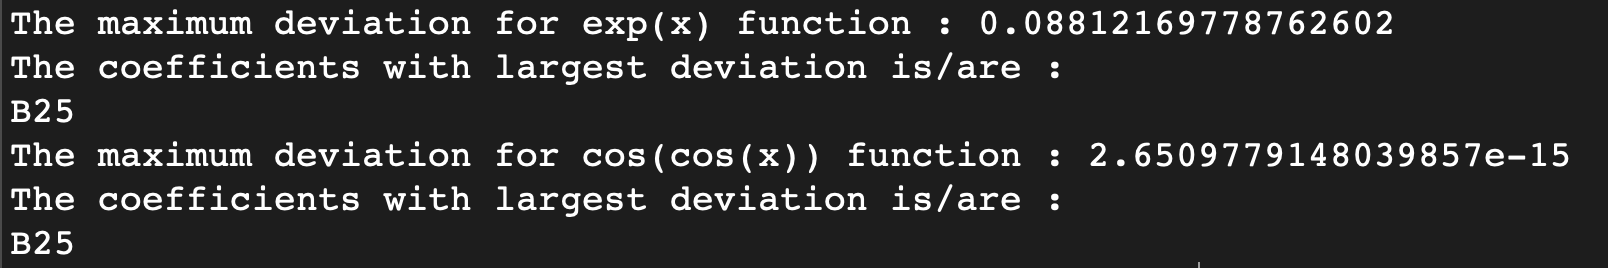
\includegraphics[scale=0.5]{out.png}
   	\label{fig:out}
   	\caption{Outputting Maximum Deviation}
\end{figure}
{We note that there is very good agreement in values in the case of $cos(cos(x))$ but a significant amount of deviation in the case of $e^{x}$. The reason for this is that the periodic extension of the exponential function is discontinuous, and hence would require a lot more higher order harmonics to accurately determine its Fourier coefficients. Also , we need more samples for Least square method to describe the discontinuous function more accurately.
\\
As we increase the number of harmonics and/or the number of samples the maximum deviation would reduce, but wouldn't reduce as significantly, and hence won't vanish.
This effect can be attributed to the \textbf{Gibbs Phenomenon}.
}
\subsection{Part 7}
The two functions are estimated using the fourier coefficients obtained via the least square method, and plotted.
\begin{minted}[tabsize = 4]{python3}
Acexp = np.matmul(A,c1)
Accos = np.matmul(A,c2)

new_x = pl.linspace(0,2*np.pi,400,endpoint = True)

pl.figure(1)
pl.title('Original and lstsq predicted versions of exp(x)')
pl.semilogy(new_x,Acexp,'go',label = 'exp(x) - Predicted')
pl.semilogy(X_list,exp(X_list),label = 'exp(x) - Original')
pl.semilogy(X_list,f1(X_list),label = 'exp(x) - Periodic Extension')
pl.xlabel(r'X $\rightarrow$')
pl.ylabel(r'Y $\rightarrow$')
pl.legend()
pl.grid(True)
pl.show()

pl.figure(2)
pl.title('Original and lstsq predicted versions of cos(cos(x))')
pl.plot(new_x,Accos,'go',label = 'cos(cos(x)) - Predicted')
pl.plot(X_list,coscos(X_list),label = 'cos(cos(x)) - Original')
pl.plot(X_list,f2(X_list),label = 'cos(cos(x)) - Periodic Extension')
pl.xlabel(r'X $\rightarrow$')
pl.ylabel(r'Y $\rightarrow$')
pl.legend()
pl.grid(True)
pl.show()
\end{minted}

{The $cos(cos(x))$ vs x graph, agrees almost perfectly, to a really good precision.
The Fourier approximation of $e^{x}$ does not agree very well to the ideal case near the discontinuity. In other places it agrees without much deviation. The cause for this is the \textbf{Gibbs Phenomenon}, which can be described as below.
\\
The partial sums of the Fourier series will have large oscillations near the discontinuity of the function. These oscillations do not die out as n increases, but approaches a finite limit.
This is one undesired phenomenon in signal processing.
\\
We can observe this phenomenon clearly when plotting the graph.
}

\begin{figure}[H]
   	\centering
   	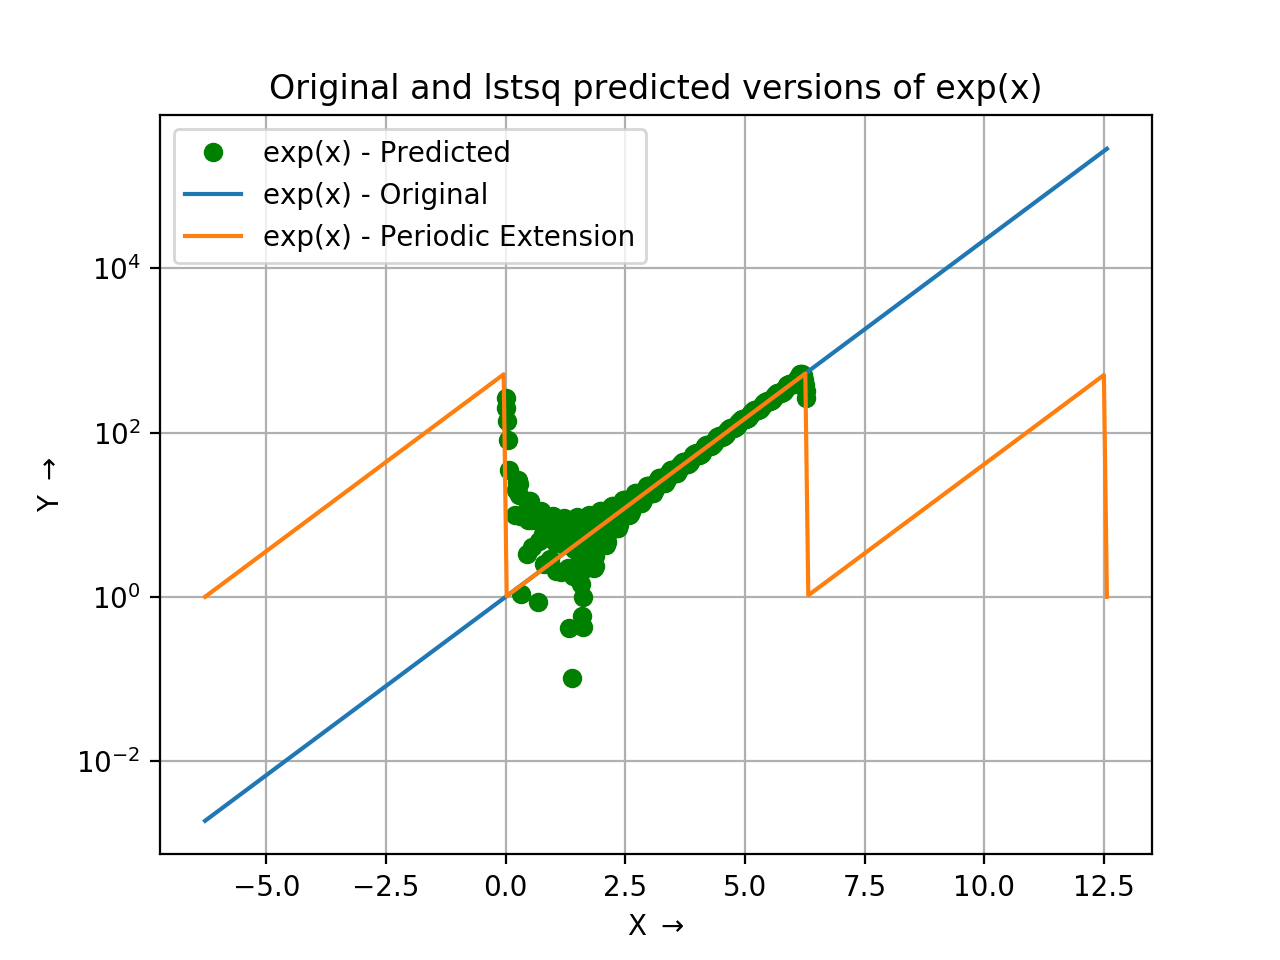
\includegraphics[scale=0.5]{expf.png}
   	\caption{$e^{x}$ vs x on a linear plot - with Least Square prediction}

   	\label{fig:expf}
\end{figure}
\begin{figure}[H]
   	\centering
   	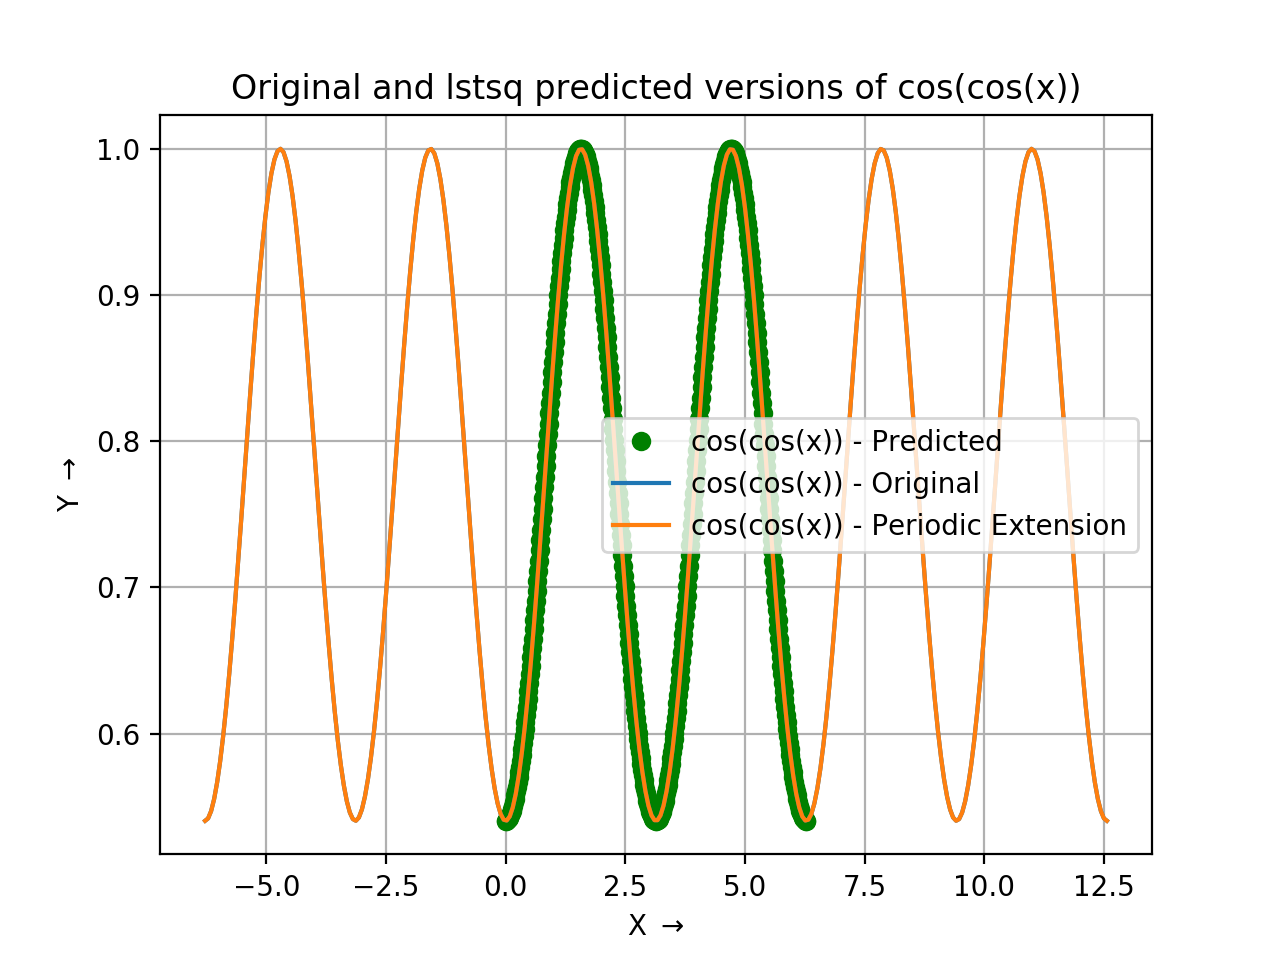
\includegraphics[scale=0.5]{cosf.png}
   	\label{fig:cosf}
   	\caption{$cos(cos(x))$ vs x on a linear plot - with Least Square prediction}

\end{figure}

\section{Conclusions}
\begin{itemize}
\item We saw two different ways of estimating the Fourier series coefficients of a periodic signal.
\item We learnt the behaviour and degree of agreement of Fourier series to continuous and discontinuous functions.
\item We observed the effect of Gibbs phenomenon at the discontinuity in the Fourier approximation of discontinuous functions.
\end{itemize}

\end{document}